\section{McClure}
\subsection{McClure: Summer 2006}
\setcounter{exercise}{0}
\setcounter{equation}{0}

\begin{problem}
  Let $X$ be a connected space and let $f\colon X\to Y$ be a function which
  is continuous and onto. Prove that $Y$ is connected. (This is a theorem
  in Munkres---prove it from the definitions).
\end{problem}
\begin{solution}
  We will show that the only separation of $Y$ is the trivial one.

  Let $C,D$ be a separation of $Y$. Then, $C$ and $D$ are open and $Y=C\cup
  D$. Since $f$ is continuous $f^{-1}(C)$ and $f^{-1}(D)$ are open in $X$
  and
  \[
    X=f^{-1}(Y)=f^{-1}(C\cup D)=f^{-1}(C)\cup f^{-1}(D).
  \]
  Since $X$ is connected we have $f^{-1}(C)=\emptyset,f^{-1}(D)=X$ or
  $f^{-1}(C)=X,f^{-1}(D)=\emptyset$; we may, without loss of generality,
  assume that $f^{-1}(C)=\emptyset$ and $f^{-1}(D)=X$. But since $f$ is
  onto, from elementary set theory, we have $f(f^{-1}(C))=C$ and
  $f(f^{-1}(D))=D$. Thus, it must be the case that $C=\emptyset$ and
  $D=Y$. It follows that the only separation of $Y$ is the trivial
  separation and so $Y$ is connected.
\end{solution}

\begin{problem}
  Let $X$ be the Cartesian product $\prod_{i=1}^\infty\bfR$ with the
  \emph{box topology} (recall that a basis for this topology consists of
  all sets of the form $\prod_{i=1}^\infty U_i$, where $U_i$ is open in
  $\bfR$). Let $f\colon\bfR\to X$ be the function which takes $t$ to
  $(t,t,\ldots)$. Prove that $f$ is not continuous.
\end{problem}
\begin{solution}
  We show that for some neighborhood $U$ of $\mathbf{0}$, $f^{-1}(U)$ is
  not open in $\bfR$ with the standard topology. Consider the set
  \[
    U=\prod_{n=1}^\infty U_n
  \]
  where $U_n=(-1/n,1/n)$. Since each $U_n$ is open in $\bfR$, $U$ is open
  in the box topology. Moreover, $\mathbf{0}\in U$ since $0\in U_n$ for all
  $n$. Therefore, $U$ is a neighborhood of $\mathbf{0}$. Now, consider the
  preimage of $U$ under $f$, $f^{-1}(U)$. We claim that
  $f^{-1}(U)=\{0\}$. We have already seen that $0\in f^{-1}(U)$ so
  $\{0\}\subset f^{-1}(U)$. It remains to show that $0$ is the only element
  in $f^{-1}(U)$. Let $x\in f^{-1}(U)$. We may, without loss of generality,
  assume that $x>0$. Then, by the Archimedean property of $\bfR$, there
  exist an natural number $N$ such that $1/N<x$. Then, for every $n\geq N$,
  $x\notin U_n$. This is a contradiction. Therefore $x\leq 0$. A similar
  argument shows that $x\geq 0$. Thus, $x=0$. Since the preimage of
  $f^{-1}(U)=\{0\}$ is not open in $\bfR$, it follows that $f$ is not
  continuous.
\end{solution}

\begin{problem}
  Let $Y$ be a topological space. Let $X$ be a set and let $f\colon X\to Y$
  be a function. Give $X$ the topology in which the open sets are the empty
  set and the sets $f^{-1}(V)$ with $V$ open in $Y$ (you do not have to
  verify that this is a topology). Let $a\in X$ and let $B$ be a closed set
  in $X$ not containing $a$. Prove that $f(a)$ is not in the closure of
  $f(B)$.
\end{problem}
\begin{solution}
  Seeking a contradiction, suppose that $f(a)\in\overline{f(B)}$. Then, for
  every neighborhood $V$ of $f(a)$, $V\cap f(B)$ is nonempty. Let
  $y\in V\cap f(B)$. Then, there exist $x\in B$ such that
  $f(x)=y$. Moreover, $f^{-1}(V)$ is, by definition, open in $X$ and is a
  neighborhood of $a$ with $x\in f^{-1}(V)\cap B$. Since every neighborhood
  of $a$ the preimage of some open subset of $Y$, it follows that $a\in
  B$. This is a contradiction. Therefore, it must be the case that
  $f(a)\notin\overline{f(B)}$.
\end{solution}

For the next two problems, let $P$ be the Cartesian product
$\prod_{i=1}^\infty\{0,1\}$ with the usual Cartesian product
topology. (Note that $\{0,1\}$ is a set with two points, it is not an
interval.)
\begin{problem}
  Prove that every function from the Cantor set $C$ to $P$ which is
  one-to-one, onto and continuous is a homeomorphism.
\end{problem}
\begin{solution}
  First, note that $P$ is Hausdorff since $\{0,1\}$ is a subspace of $\bfR$
  which is Hausdorff and the product of Hausdorff spaces equipped with the
  product topology is again Hausdorff.

  Moreover, since $C=\bigcap_{n=1}^\infty A_n$ and each $A_n$ is the
  disjoint union of a finite collection of closed intervals in $[0,1]$, $C$
  is closed since the intersection of a collection of closed sets is again
  closed. Then $C$ is compact since it is a closed subspace of $[0,1]$, the
  latter a compact subspace of $\bfR$.

  It follows from a theorem in chapter 23 that if $f\colon C\to P$ is
  one-to-one, onto and continuous it is a homeomorphism since $C$ is
  compact and $P$ is Hausdorff.
\end{solution}

\begin{problem}
  \hfill
  \begin{enumerate}[label=(\alph*),noitemsep]
  \item Give a clear and specific description of a function from the Cantor
    set to $P$ which is one-to-one and onto. You do not have to prove that
    your function is one-to-one and onto.
  \item Prove that the function you described in part (a) is
    continuous. (If it isn't continuous, go back and choose a different
    function that is).
  \end{enumerate}
\end{problem}
\begin{solution}
  For part (a) we take the following claim will be taken for granted: The
  set $C$ consists of all term series of the form
  \[
    \sum_{n=1}^\infty\frac{a_n}{3^n}
  \]
  where $a_n\in\{0,2\}$. Define a map $f\colon C\to P$ by
  \[
    f\left(\sum_{n=1}^\infty\frac{a_n}{3^n}\right)=(a_1/2,a_2/2,\ldots).
  \]

  For part (b), to see that $f$ is continuous note that
  $\pi_n\circ f=a_n/2$ is multiplication on $\bfR$ which is continuous on
  $\bfR$, hence it is continuous on the subspace $\{0,1\}$ of $\bfR$. By
  the universal mapping property of the product topology (see the diagram
  below)
  \[
    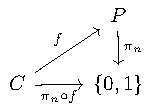
\includegraphics{aug06/aug06-prob5}
  \]
  since every projection of $f$, $\pi_n\circ f$ is continuous, it follows
  that $f$ is continuous.
\end{solution}

\begin{problem}
  Let $X$ and $Y$ be topological spaces, let $x_0\in X$, $y_0\in Y$ and let
  $f\colon X\to Y$ be a continuous function which takes $x_0$ to $y_0$.

  Is the following statement true? If $f$ is one-to-one then
  $f_*\colon\pi(X,x_0)\to \pi_1(Y,y_0)$ is one-to-one. Prove or give a
  counterexample (and if you give a counterexample, justify it). You may
  use anything in Munkres's book.
\end{problem}
\begin{solution}
  We provide a counter example. Let $B^2$ be the open ball of radius $1$
  cenntered at $(0,0)$, $S^1$ the circle of radius $1$ centered at $(0,0)$
  and fix $x_0=(0,1)$ on $S^2$ Then, the canonical inclusion
  $\iota\colon S^1\to B^2$ is injective. However, $\pi_1(S^1,x_0)\cong\bbZ$
  whereas $\pi_1(B^2,x_0)\cong \{0\}$ and no map $f\colon\bbZ\to\{0\}$ is
  injective.
\end{solution}

\begin{problem}
  Let $S^2$ be the $2$-sphere, that is, the following subspace of $\bfR^3$:
  the set
  \[
    \left\{\,(x,y,z)\in\bfR^3:x^2+y^2+z^2=1\,\right\}.
  \]
  Let $x_0$ be the point $(0,0,1)$ of $S^2$.


  Use the Seifert--van Kampen theorem to prove that $\pi_1(S^2,x_0)$ is the
  trivial group. You may use either of the two versions of the Seifert--van
  Kampen theorem given in Munkres's book. You will not get credit for any
  other method.
\end{problem}

\begin{solution}
  Let $N$ and $S$ denote the points $(0,0,1)$ and $(0,0,-1)$,
  respectively. Then the sets
  \[
    U=S^2\setminus\{N\}\qquad\text{and}\qquad V=S^2\setminus\{S\}
  \]
  are open in $S^2$ and both contain the point $x_0$. Now since
  $U,V\approx\bfR$ via the stereographic projections
  $\pi_N\colon N\to\bfR^2$, $\pi_S\colon S\to\bfR^2$ we have
  \[
    \pi_1(U,x_0)\cong\pi_1(V,x_0)\cong\pi_1(\bfR^2,\pi_N(x_0))\cong 0.
  \]
  Thus, by the Seifert--van Kampen theorem,
  \[
    \pi_1(S^2,x_0)\cong\frac{\pi_1(U,x_0)*\pi_1(V,x_0)}{N'}\cong 0
  \]
  since $0*0\cong 0$ and any quotient of the trivial subgroup is trivial.
\end{solution}

%%% Local Variables:
%%% mode: latex
%%% TeX-master: "../MA571-Quals"
%%% End:
